We initially configured the Reservation Station (RS) size to 8. However, this setup resulted in a high structural hazard rate of approximately 28\%, which prevented instructions from being dispatched. These stalls contributed to an increased CPI due to underutilization of functional units and pipeline inefficiency.
\begin{figure}[htbp]
  \centering
  \begin{minipage}[t]{0.24\textwidth}
    \centering
    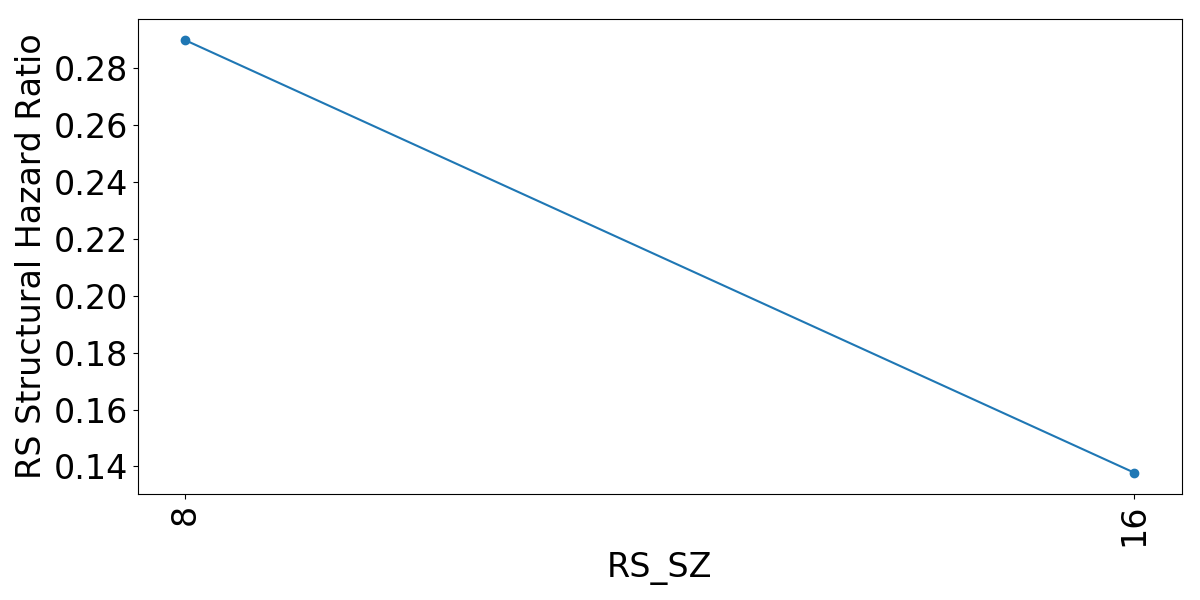
\includegraphics[width=\textwidth]{figures/Analysis/N-way/RS_Stru.png}
    \caption{RS Size vs. RS Full Rate}
    \label{fig:rs_stall}
  \end{minipage}
  \hfill
  \begin{minipage}[t]{0.24\textwidth}
    \centering
    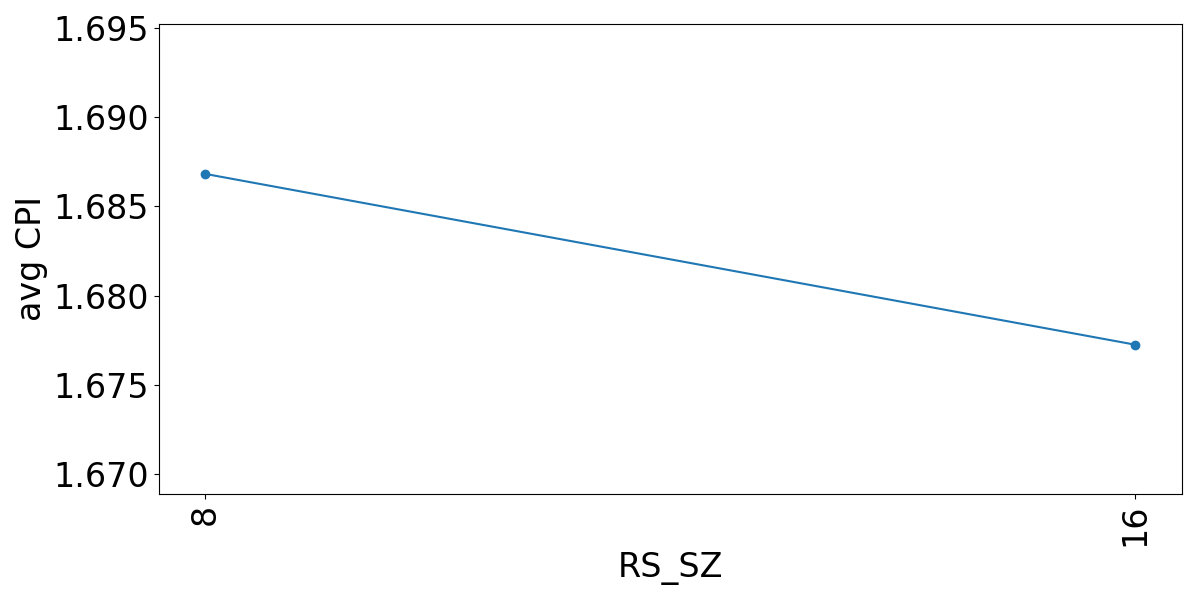
\includegraphics[width=\textwidth]{figures/Analysis/N-way/cpi_RS.png}
    \caption{RS Size vs. CPI}
    \label{fig:rs_cpi}
  \end{minipage}
\end{figure}
To alleviate this issue, we increased the RS size to 16. As shown in Figure~\ref{fig:rs_stall}, this optimization reduced the structural hazard rate by more than 50\% and as shown in Figure~\ref{fig:rs_cpi}, the reduction in CPI was about 0.5\%.